\documentclass[a4paper,12pt]{article}
\usepackage{../../../mypackages}
\usepackage{../../../macros}


\usepackage{pgfplots}
    \pgfplotsset{
    compat=1.11,
  }

\setlength{\parindent}{0pt}


\begin{document}

\title{Chapitre 1 - Les fonctions}
\author{N. Bancel}

\maketitle

\section*{Les fonctions}



\subsection*{Les fonctions polynomes de degré 2}

On appelle fonction polynôme de degré 2, toute fonction de la forme :
\[
    f(x) = ax^2 + bx + c
\]

%\(f(x) = -x^2 + 4x + 12\)

où $a$, $b$ et $c$ sont des nombres réels, et $a$ doit être non nul.

Cette fonction peut parfois s'écrire sous la forme : 
\[
    f(x) = a(x - x_1)(x - x_2)
\]

avec $x_1$ et $x_2$ des nombres réels et $a$ non nul.

\begin{itemize}[noitemsep]
  \item Dans le premier cas on parlera de \textit{forme développée}
  \item Dans le second de \textit{forme factorisée}.
\end{itemize}


\textbf{\textcolor{blue}{Exemple}} \par 

Montrer que l'on peut réécrire la fonction $f(x) = 3x^2 - 15x + 18$ sous la forme $f(x) = 3(x - 3)(x - 2)$

\subsection*{Racines d'un polynôme du 2nd degré}

On appelle racine d'un polynôme du second degré les solutions de l'équation :
\[
    ax^2 + bx + c = 0
\]
Dans le cas où le polynôme est donné sous forme factorisée :
\[
    a(x - x_1)(x - x_2)
\]
les racines seront $x_1$ et $x_2$.


\textbf{\textcolor{blue}{Exemple}} \par

\begin{itemize}[noitemsep]
  \item Quelles sont les racines du polynôme $-4(x - 5)(x + 1)$ ?
  \item 2 est-il racine de \(x^2 - 3x + 7\) 
\end{itemize}

\subsection*{Trouver la forme factorisée à partir d'une racine}

Si une racine est donnée, on peut trouver la seconde par identification.

\textbf{\textcolor{blue}{Exemple}} \par 

Factoriser $-4x^2 + 16x + 20$ sachant que -1 est une racine.

On sait d'après l'énoncé que :

\[
-4x^2 + 16x + 20 = -4(x + 1)(x - \alpha)
\]

où $\alpha$ est la seconde racine que nous cherchons.

Si nous développons $-4(x + 1)(x - \alpha)$, nous obtenons :

\begin{align}
  -4(x + 1)(x - \alpha) &= -4(x^2 - \alpha x + x - \alpha) \\
  &= -4(x^2 + x(1 - \alpha) - \alpha) \\
  &= -4x^2 - 4x(1 - \alpha) - 4\alpha
\end{align}

Par identification des coefficients, on s'aperçoit que :


\begin{equation*}
\begin{cases}
    -4(1 - \alpha) = 16  \\
    4\alpha = -20 
\end{cases}
\end{equation*}

On peut utiliser l'une des équations pour trouver $\alpha$ : la seconde, par exemple, nous donne : $\alpha = \frac{20}{-4} = -5$. On en déduit que la seconde racine est $-5$.

\section*{Représentation graphique}

\subsection*{La fonction parabolique}


On considère la fonction polynôme du second degré :

\[
f(x) = ax^2 + bx + c
\]

La représentation graphique d'une fonction polynôme du second degré est une parabole.

— Le sens de variation de $f$ dépend uniquement du signe de $a$. \\
— Le signe de $f$ dépend du signe de $a$ ainsi que des racines de $f$.

\subsection*{Sommet et axe de symétrie}

La fonction polynôme du second degré admet pour axe de symétrie $x = -\frac{b}{2a}$ (forme développée) ou $x = \frac{x_1 + x_2}{2}$ (forme factorisée).

\begin{figure}[H]
  \centering
  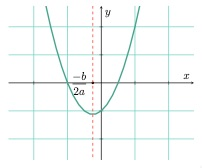
\includegraphics[width=0.3\linewidth]{symetrie.jpg}
  \caption{\label{} Symétrie d'une parabole}
\end{figure}

Son sommet a pour coordonnées $\left(-\frac{b}{2a}, f\left(-\frac{b}{2a}\right)\right)$.

\subsection*{Tableau de variation}

\begin{tikzpicture}
  \tkzTabInit[lgt=3]
  {$x$ / 1 , \(f(x)\) avec a > 0 / 3, \(f(x)\) avec a < 0 / 3 }{$-\infty$, $-\frac{b}{2a}$, $+\infty$}
  \tkzTabVar{+/$+\infty$,-/$f(-\frac{b}{2a})$,+/$+\infty$}
  \tkzTabVar{-/$-\infty$,+/$f(-\frac{b}{2a})$,-/$-\infty$}
  %\tkzTabVar{+/$+\infty$,-/$0$,+/$+\infty$}
\end{tikzpicture}

\subsection*{Pause exercices}

\begin{tcolorbox}
Notions à intégrer

\begin{itemize}[noitemsep]
  \item[$\bullet$] Appartenance d'un point à une courbe
  \item[$\bullet$] Résolution graphique d'équation
  \item[$\bullet$] Racines de polynomes
\end{itemize}

\end{tcolorbox}

Faire les exercices 13, 14, 28, 31, 37, Questions 1 et 2 de l'exercice 47



\section*{Résolution d'inéquation du 2nd degré}

\subsection*{Tableau de signe}

Si \(f\) a deux racines :

\begin{tikzpicture}
  \tkzTabInit{$x$ / 1 , $f(x)$ / 1}{$-\infty$, $x_1$, $x_2$, $+\infty$}
  \tkzTabLine{, \text{signe de } a, z, \text{signe de } -a, z, \text{signe de } a}
\end{tikzpicture}

Si \(f\) a 1 racine :

\begin{tikzpicture}
  \tkzTabInit{$x$ / 1 , $f(x)$ / 1}{$-\infty$, $x_1$, $+\infty$}
  \tkzTabLine{, \text{signe de } a, z, \text{signe de } a}
\end{tikzpicture}

Si \(f\) n'a pas de racine :

\begin{tikzpicture}
  \tkzTabInit{$x$ / 1 , $f(x)$ / 1}{$-\infty$, $+\infty$}
  \tkzTabLine{, \text{signe de } a}
\end{tikzpicture}

\textbf{\textcolor{blue}{Exemple}} \par 

\begin{itemize}[noitemsep]
  \item[$\bullet$] Donner le tableau de signe de la fonction $f(x) = -4(x-2)(x+3)$
  \item[$\bullet$] Résoudre l'inéquation $-4(x-2)(x+3) \leq 0$
\end{itemize}

\section*{Fonction polynôme de degré 3}

\subsection*{Définition}

On appelle fonction polynôme de degré 3, toute fonction de la forme :

\[
f(x) = ax^3 + bx^2 + cx + d
\]

où $a$, $b$, $c$ et $d$ sont des réels et $a$ est non nul.

\textbf{\textcolor{blue}{Exemple}} \par

La fonction $f(x) = 5x^3 + 4x^2 + 3$ est une fonction polynôme de degré 3.

\subsection*{Forme développée et forme factorisée}

Tout comme pour les fonctions polynômes de degré 2, une fonction polynôme de degré 3 peut éventuellement s'écrire sous forme factorisée :

\[
f(x) = a(x - x_1)(x - x_2)(x - x_3)
\]

avec $a$, $x_1$, $x_2$ et $x_3$ des nombres réels et $a$ est non nul.

\textbf{\textcolor{blue}{Exemple}} \par

Montrer que l’on peut réécrire la fonction $f(x) = 2x^3 - 2x^2 - 20x - 16$ sous la forme :

\[
f(x) = 2(x - 4)(x + 2)(x + 1)
\]

\textbf{Réponse:}

\begin{align}
  2(x - 4)(x + 2)(x + 1) = 2(x - 4)(x^2 + x + 2x + 2) &= 2(x - 4)(x^2 + 3x + 2) \\
  &= 2(x^3 + 3x^2 + 2x - 4x^2 - 12x - 8) \\
  &= 2(x^3 - x^2 - 10x - 8) \\
  &= 2x^3 - 2x^2 - 20x - 16
\end{align}

\textbf{Remarque:} Un polynôme de degré 3 n’a pas forcément une forme factorisée.

\subsection*{Racines d’un polynôme de degré 3}

On appelle racines d’un polynôme de degré 3 les solutions de l’équation : $ax^3 + bx^2 + cx + d = 0$. Dans le cas où le polynôme est donné sous forme factorisée $a(x - x_1)(x - x_2)(x - x_3)$, les racines seront $x_1$, $x_2$ et $x_3$.

\subsection*{Tableau de signes de $a(x - x_1)(x - x_2)(x - x_3)$}

Dans le cas où la fonction polynôme de degré 3 a trois racines, son tableau de signes sera :

\end{document}



